\chapter{Containerisierung mit Docker}
Im Folgenden werden Docker, die Bestandteile von Docker und der Unterschied zwischen Virtualisierung und Containerisierung erklärt.
Anschließend wird auch die Notwendigkeit von Containerisierung für Cloud-Plattformen aufgezeigt.

\section{Docker}
Docker ist ein Container-Management-System, das es erleichtert, Linux Container zu managen. Docker erlaubt das Erstellen von Docker Images in virtuellen Umgebungen am lokalen PC. Auf diesen Umgebungen können Kommandos und Operationen ausgeführt werden. Diese Aktionen unterscheiden sich am lokalen PC nicht von den Aktionen am Produktivsystem. Dies hilft bei der Entwicklung lokal sowie beim Deployment auf der Produktivumgebung am Server, da die auszuführenden Kommandos dieselben sind \cite{MasteringDocker}.

\subsection{Komponenten von Docker}
Im Folgenden werden die Kernkomponenten von Docker beschrieben.

\subsubsection{Docker Engine}
Docker ist eine Client-Server Anwendung. Der Docker-Server wird auch als \textit{Docker Daemon} oder \textit{Docker Engine} bezeichnet. Bei der Installation von Docker werden eine Command Line Binary und eine RESTful API mitgeliefert, um mit dem Docker Daemon zu interagieren. Der Docker Daemon und der Docker Client können am selben Host laufen. Der lokale Docker Client kann aber auch mit einem Remote Docker Daemon verbunden werden.
Der Docker Daemon erzeugt und managt die Docker Container am Docker Host. Die Kommunikation des Docker Client mit dem Docker Daemon läuft über die von Docker bereitgestellte REST-API. \cite{TheDockerBook}

\subsubsection{Docker Images}
Docker Images sind die Bausteine im Docker System. Docker Container werden aus Docker Images gestartet. Docker Images sind mehrschichtig und werden schrittweise mittels einer Serie von Instruktionen erstellt.
Beispiele für solche Instruktionen sind:
\begin{itemize}
	\item eine Datei hinzufügen,
	\item einen Befehl im Container ausführen,
	\item einen Port öffnen.
\end{itemize}

Docker Images werden auch als \glqq Source Code\grqq{} für Container bezeichnet. Docker Images sind sehr portabel und können einfach verbreitet, gespeichert und aktualisiert werden \cite{TheDockerBook}. 

Die Instruktionen zum Bauen eines Docker Image werden in einem \textit{Dockerfile} beschrieben. Kommandos, Aufrufe von Scripts, das Setzen von Environment-Variablen, das Hinzufügen von Dateien und das Setzen von Rechten können alle im Dockerfile beschrieben werden. Im Dockerfile muss auch das Basisimage für den Build spezifiziert werden. Ein Dockerfile sieht beispielsweise wie in Listing \ref{lst:BSPDockerfile} dargestellt aus \cite{MasteringDocker}:

\begin{lstlisting}[language=docker, caption=Beispiel für ein Dockerfile, label={lst:BSPDockerfile}]
	FROM ubuntu:latest
	MAINTAINER Scott P. Gallagher <email@somewhere.com>
	
	RUN apt-get update && apt-get install -y apache2
	
	ADD 000-default.conf /etc/apache2/sites-available
	RUN chown root:root /etc/apache2/sites-available/000-default.conf
	
	EXPOSE 80
	CMD ["/usr/sbin/apache2ctl", "-D", "FOREGROUND"]
\end{lstlisting}

Dies sind typische Befehle, die in den meisten Dockerfiles zu finden sind. Im \textit{FROM}-Befehl wird das Basisimage, auf dem das Docker Image aufgebaut ist, definiert. Jede weitere Zeile fügt eine neue  Schicht im Docker Image hinzu. Mit dem Befehl:
\begin{lstlisting}[language=bash]
$ docker build <DOCKERFILE>
\end{lstlisting}
kann dieses Docker Image gebaut werden. Aus diesem Docker Image kann danach ein Docker Container erzeugt werden \cite{MasteringDocker}.

\subsubsection{Registries}
Die gebauten Docker Images werden in Registries gespeichert. Dabei gibt es zwei verschiedene Arten von Registries: \textbf{public} und \textbf{private}. Docker, Inc., verwaltet die public Registry, auch \href{https://hub.docker.com/}{Docker Hub} genannt. In der public Registry befinden sich auch bereits vordefinierte Docker Images für zum Beispiel eine MySQL-Datenbank oder einen Nginx Webserver.
Es kann auch eine eigene private Registry erstellt werden. Diese erlaubt das Speichern von Images, ohne dass von außen auf diese zugegriffen werden kann \cite{TheDockerBook}.

\subsubsection{Docker Container}
In Docker Containern können Applikationen und Services laufen. Docker Container werden aus Docker Images erstellt und können einen oder mehrere Prozesse enthalten. 
Ein Docker Container besteht aus \cite{TheDockerBook}:

\begin{itemize}
	\item einem gebauten Docker Image,
	\item einem Set von Standardoperationen,
	\item einer Umgebung zum Ausführen der Operationen.
\end{itemize}

Jeder Docker Container enthält ein Software Image, dass das Erstellen, Starten, Stoppen, Neustarten und Löschen des Docker Containers erlaubt. Docker kümmert sich dabei nicht um den Inhalt des Containers. Jeder Container, egal ob eine MySQL-Datenbank oder ein Nginx Webserver, wird gleich gestartet oder gelöscht.
Docker ist dabei unabhängig von der Umgebung in, der der Docker Container läuft. Es kann lokal am PC gebaut, in die public Registry hochgeladen werden oder der Container in der Cloud laufen. Dadurch kann mit Docker schnell ein Application Server, ein Message Bus oder ein Continous-Integration-Test erstellt und getestet werden \cite{TheDockerBook}.

\subsection{Unterschied zwischen Virtualisierung und Containerisierung}
\subsubsection{Virtualisierung}
Eine virtuelle Maschine, welche die Virtualisierung auf Hardware-Level repräsentiert, ist grundsätzlich ein komplettes Operating System, das in einem Host Operating System läuft. Dabei gibt es zwei Arten von \glqq Virtualization Hypervisors\grqq: \textbf{Type 1} und \textbf{Type 2}. Type 1 Hypervisors bieten Server-Virtualisierung auf Hardware-Level. Dabei gibt es kein traditionelles End-User Operating System.
Type 2 Hypervisors werden zur Desktop Virtualisierung verwendet. Die Virtualisierungs-Engine läuft dabei auf einem eigenen Operating System. Der größte Vorteil von virtuellen Maschinen ist, dass mehrere unterschiedliche Operating Systeme auf einem Host laufen können \cite{DevelopingWithDocker}.

Virtuelle Maschinen sind voll isoliert und daher sehr sicher. Sie enthalten jedoch alle Bestandteile, die ein Operating System aufweisen muss: Treiber, Systembibliotheken, etc.
Virtuelle Maschinen sind daher sehr schwergewichtig und ressourcenhungrig. Auch die Installation virtueller Maschinen ist sehr komplex und aufwändig. Um eine Applikation in einer virtuellen Maschine zu starten, muss der Hypervisor die virtuelle Maschine zuerst importieren und danach starten. Weiters können nur wenige virtuelle Maschinen auf einer einzelnen Maschine gestartet werden, da die Performanz mit jeder neuen virtuellen Maschine drastisch abnimmt \cite{DevelopingWithDocker}.

\subsubsection{Containerisierung}
Abbildung \ref{fig:DOC_DockerVSTraditional} zeigt einen der größten Vorteile von Docker. Docker benötigt kein neues Betriebssystem, sobald ein neuer Container gestartet wird. Dies verringert die Größe der einzelnen Container drastisch. Docker baut dabei auf den Linux Kernel des Host OS auf. Dies macht es möglich, jedes Linux OS als Host OS zu verwenden. Beispielsweise kann auf der linken App in der Abbildung auf der Dockerseite Red Hat laufen und auf der anderen Debian. Dazu muss weder Red Hat noch Debian auf dem Host installiert sein.
Docker Images werden dadurch so klein wie möglich gehalten. Sie sind dadurch sehr kompakt und einfach zu deployen \cite{MasteringDocker}.

Docker Container sind nicht nur vom darunterliegenden Operating System isoliert, sondern auch von anderen Docker Containern. Die Startzeiten von Docker Containern sind in der Regel durch den geringen Overhead sehr schnell. Docker Container ersetzen jedoch virtuelle Maschinen nicht ganz. Es muss vor der Entwicklung evaluiert werden, welches Vorgehen die beste Wahl ist. Auf der einen Seite gibt es völlig isolierte, sichere virtuelle Maschinen mit durchschnittlicher Performanz und auf der anderen Seite hoch performante, schnell deploybare Docker Container \cite{DevelopingWithDocker}.

\begin{figure}[H]
	\begin{center}
		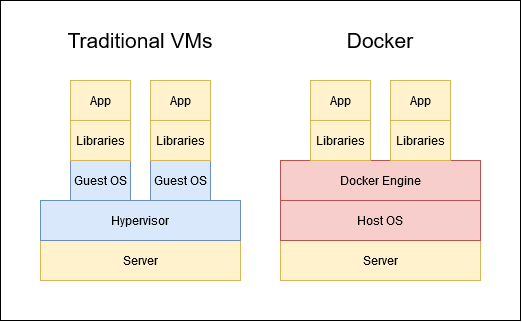
\includegraphics[scale=0.65]{DockerVSTraditional.png}
		\caption[Unterschied von traditionellen VMs zu Docker]{Unterschied von traditionellen VMs zu Docker \cite{MasteringDocker}}
		\label{fig:DOC_DockerVSTraditional}
	\end{center}
\end{figure}

\subsection{Vorteile von Docker}
In diesem Abschnitt werden die Vorteile von Docker und Containerisierung im Gegensatz zu virtuellen Maschinen und Virtualisierung beschrieben.

\subsubsection{Schnelligkeit und Größe}
Docker Container können schnell und einfach erstellt und wieder gelöscht werden. Docker teilt sich nur den Kernel mit dem Operating System. Auch Schichten von Docker Images können wiederverwendet werden. Dies führt zu sehr leichtgewichtigen Docker Containern. Die Resultate sind schnelles Deployment, einfache Migration und kurze Startzeiten \cite{DevelopingWithDocker}.

\subsubsection{Reproduzierbarkeit und portable Builds}
Docker erlaubt das Deployment von ready-to-use Software, welche portabel und sehr einfach zu verteilen ist. Die containerisierte Applikation läuft im Docker Container, daher wird keine Installation benötigt. Docker Images definieren alle Abhängigkeiten, die das System benötigt. Dies verringert Fehler mit Versionskonflikten und Kompatibilität. Entwickler können dasselbe Docker Image, das in der Produktionsumgebung läuft, lokal testen. Dies verschnellert auch den Prozess der Continous Integration. Es gibt keine endlosen Build-Test-Deploy-Zyklen. Docker stellt dabei sicher, dass sich die Applikationen in Entwicklungs-, Test- und Produktionsumgebungen ident verhalten \cite{DevelopingWithDocker}.

Die Portabilität ist eine der größten Stärken von Docker. Docker Container können fast überall deployt und gestartet werden: am lokalen PC, am weit entfernten Server oder auf der privaten oder öffentlichen Cloud.
Nahezu alle Cloud Computing-Provider unterstützen Docker als Containerisierungsplattform. Ein Docker Container, der z.B. auf einer Amazon EC2-Instanz läuft, kann sehr einfach auf einer Google Compute Engine-Instanz deployt werden. Durch den zusätzlichen Level an Abstraktion funktioniert Docker sehr gut mit vielen unterschiedlichen Cloud Providern \cite{DevelopingWithDocker}. 

\subsubsection{Unveränderbare und agile Infrastruktur}
Eine idempotente Codebasis speziell im Bereich Konfigurationsmanagement zu warten ist sehr komplex und zeitintensiv. Die Codebasis wächst und wird immer komplexer. Deshalb wird unveränderbare Infrastruktur immer wichtiger. Containerisierung hilft dabei ungemein. Durch die Verwendung von Containern wird der Prozess des Entwickelns und des Deployments vereinfacht. Docker benötigt wenig Konfigurationsmanagement. Die Applikationen werden durch einfaches Deployment und Redeployment gemanagt. 
Docker bietet durch vorgefertigte Docker Images den Großteil der Konfiguration. Diese vorgefertigten Docker Images können mittels einem Dockerfile erweitert werden. Docker folgt dabei dem Ansatz \textit{Infrastructure as Code}, wo die Infrastruktur des Servers als Code vorliegt. Bei Docker ist dies das Dockerfile \cite{DevelopingWithDocker}.

\subsubsection{Tools und APIs}
Docker ist nicht nur ein Dockerfile-Prozessor und eine Runtime Engine. Docker ist ein komplettes Paket mit einer Vielzahl an Tools und APIs. Die Docker Toolbox ist ein Installer, um schnell und einfach eine Docker-Umgebung auf dem eigenen Rechner zu installieren. \textit{Kinematic} ist eine Desktop-Entwicklerumgebung zur Verwendung von Docker auf Windows und Mac OS X Rechnern. Docker enthält auch eine Vielzahl an Kommandozeilentools zur Entwicklung von Applikationen mit Docker \cite{DevelopingWithDocker}.

\section{Notwendigkeit von Containerisierung}
Containerisierung ist gerade bei Cloud Plattformen, wie OpenShift, sehr wichtig. Durch die Instanzierung eines Image wird ein Container erzeugt. In diesem läuft die Applikation.
Applikationen, die in einem Container laufen, sind sicherer als Applikationen, die nicht in einem Container laufen. Container nutzen dabei die Sicherheit des Linux Kernel Namespace, um Applikationen, die am selben Rechner und unter denselben \textbf{control groups (cgroups)} laufen, zu sandboxen. Dabei wird dem Risiko, dass eine Applikation alle Ressourcen eines Servers nutzt, entgegengewirkt. Einem Container kann eine maximale Verwendung von CPU-Ressourcen zugewiesen werden. Dadurch wird sichergestellt, dass alle Anwendungen genug Ressourcen bekommen \cite{GettingStartedWithContainerization}.

Dadurch, dass die Images unveränderbar sind, können sie auch auf mögliche Angriffsstellen und Veralterung überprüft werden.
Weiters kann auch \textbf{content trust} verwendet werden. Dabei wird sichergestellt, dass der Ersteller des Image auch wirklich derjenige ist, der er vorgibt zu sein. Dadurch werden die Images auch gegen \textbf{man-in-the-middle}-Attacken gesichert, wo während dem Versenden das Image ohne Wissen des Empfängers geändert wird \cite{GettingStartedWithContainerization}.

Durch die Containerisierung kann auch einfach am PC des Entwicklers eine produktionsähnliche Umgebung geschaffen werden. Dadurch, dass jede Applikation containerisiert werden kann, können auch z.B. Datenbanken, wie Oracle oder MS SQL Server, schnell für die lokale Entwicklung verwendet werden. Diese müssen dann nicht am PC des Entwicklers aufwändig installiert und konfiguriert werden \cite{GettingStartedWithContainerization}.

Container sind auch schneller und einfacher zu erstellen, zu deployen und zu managen als virtuelle Maschinen. Container benötigen auch weniger Rechenleistung. Daher ist es möglich, mehrere Container am selben Rechner laufen zu lassen. Dies spart natürlich auch Kosten beim Hosten von Applikationen in der Cloud \cite{GettingStartedWithContainerization}.

Ein weiterer wichtiger Punkt ist das Aufsetzen und Hochfahren der gesamten Applikation von z.B. Projektleitern bei Präsentationen beim Kunden. Projektleiter sind oft bei der eigentlichen Entwicklung der Anwendung nicht involviert und haben deshalb die Infrastruktur am eigenen Rechner nicht eingerichtet. Durch die schnelle und einfache Verwendung von Docker ist es für Projektleiter um einiges einfacher, die Software beim Kunden zu präsentieren \cite{GettingStartedWithContainerization}.